\documentclass[]{article}
\usepackage{graphicx}
\usepackage{amsmath}
%opening
\title{CSC420 Assignment 2}
\author{Alex (Kao-Tsun) Chang}


\begin{document}

\maketitle


\section{}
\textbf{(a)}
\begin{figure}[h!]
\centering
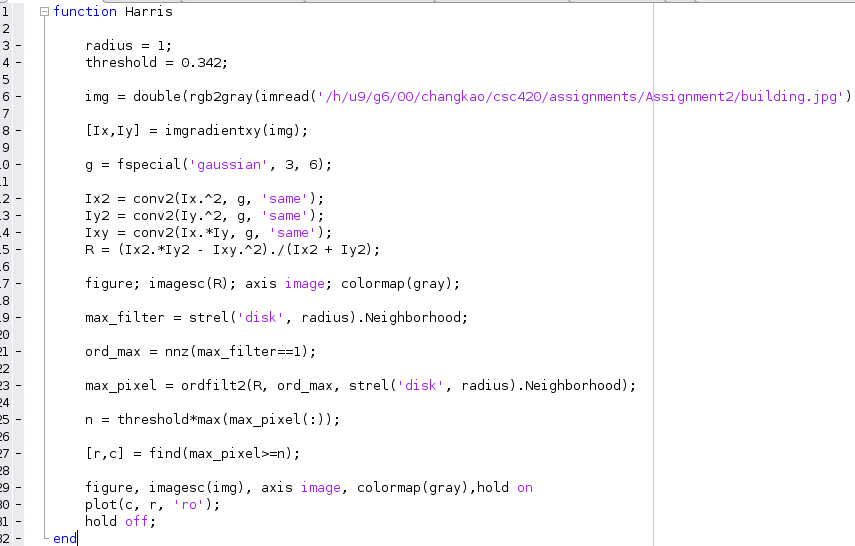
\includegraphics[width=1.35\textwidth]{img/1a-code.png}
\caption{Harris Corner w/ maximal suppression}
\end{figure}
\begin{figure}[h!]
\centering
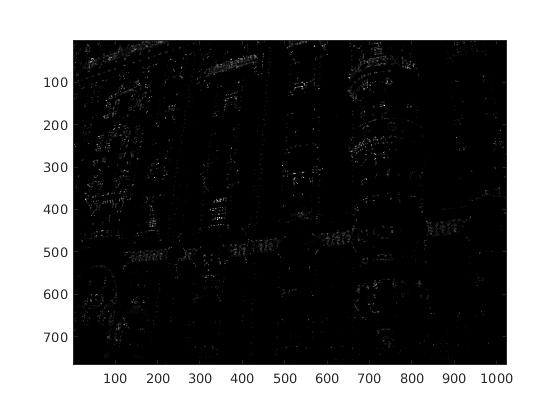
\includegraphics[width=1.15\textwidth]{img/1a.jpg}
\caption{Output}
\end{figure}


.\\\\\\
\textbf{(b)}
With a bigger r, the interest point is compared with a bigger area during non-max suppression, thus it is more likely to be pruned during non-max suppression, thus less interest points as r increases.
\begin{figure}[h!]
\centering
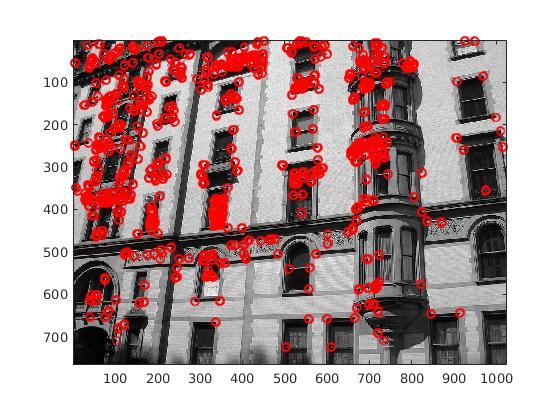
\includegraphics[width=1.35\textwidth]{img/1a-2.jpg}
\caption{output w/ threshold = 0.342; r = 1}
\end{figure}

.\\\\\\\\\\\\\\\\
\begin{figure}[h!]
\centering
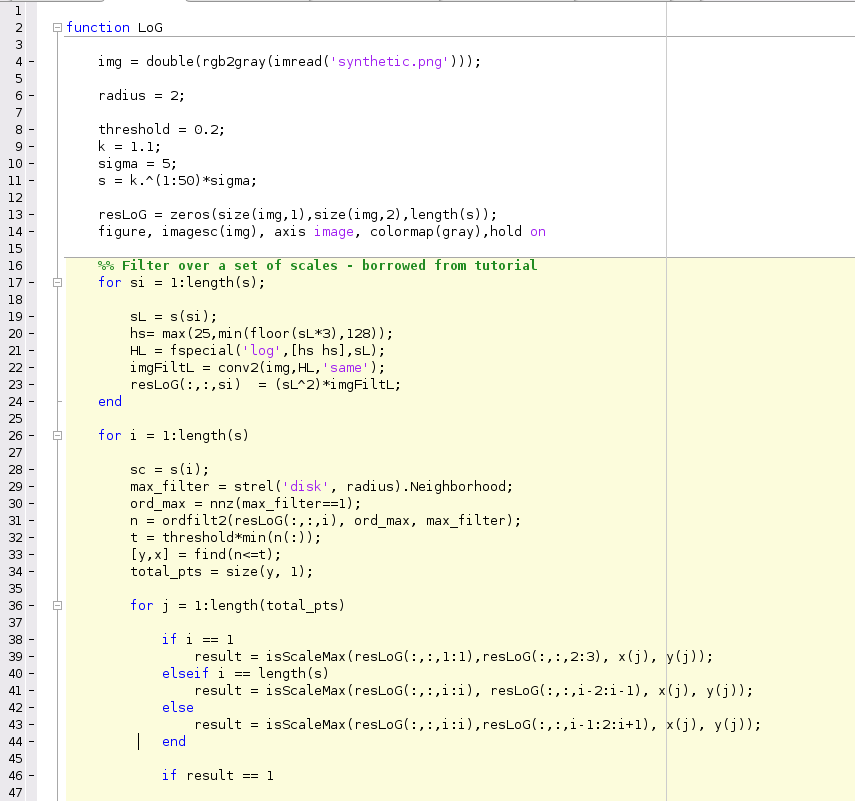
\includegraphics[width=1.35\textwidth]{img/1c1-code.png}
\caption{Laplacian matlab code}
\end{figure}

\begin{figure}[h!]
\centering
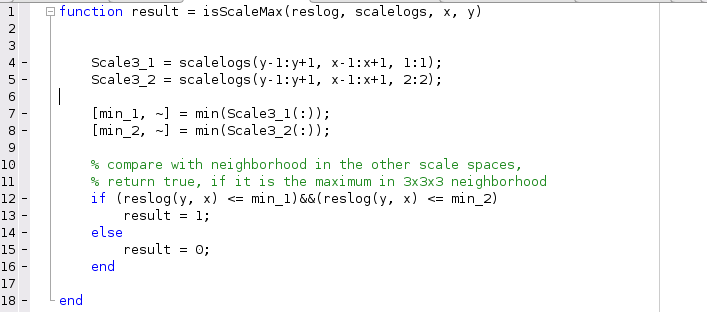
\includegraphics[width=1.35\textwidth]{img/1c3-code.png}
\caption{Laplacian helper function - isScaleMax matlab code}
\end{figure}

\begin{figure}[h!]
\centering
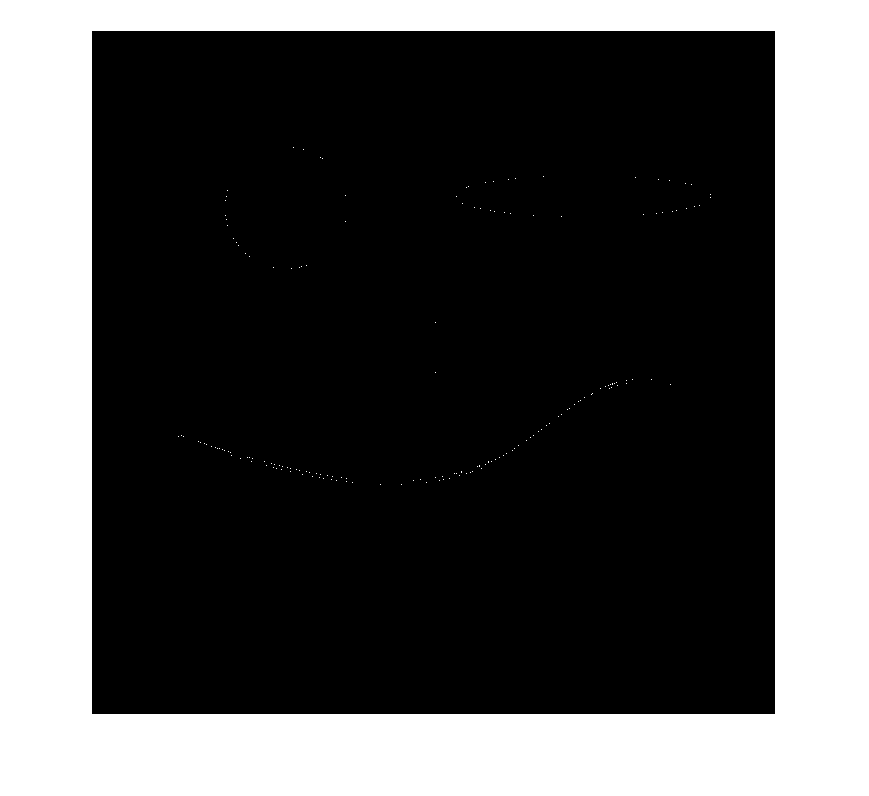
\includegraphics[width=1.35\textwidth]{img/1c-output.png}
\caption{Laplacian output}
\end{figure}
.\\\\\\\\\\\\\\\\\\\\\\\\\\\\\\\\\\\\\\\\\\\\\\\\\\\\\\\\\\\\\\\\\\\\\\\\\\\\\\\\\\\\\\\\\\\\\\\\\\\\\\\\\\\\\\\\\\
\textbf{(d)}

The Harris detector and Laplacian detector seems to be able to detect sharp edge corners well, as well as the corners detected were all similar in size.
\\ The difference between the two were that the Laplacian was able to detect rounded edges and circles better then the harris corner detector


\section{}
\textbf{(a)}

\begin{figure}[h!]
\centering
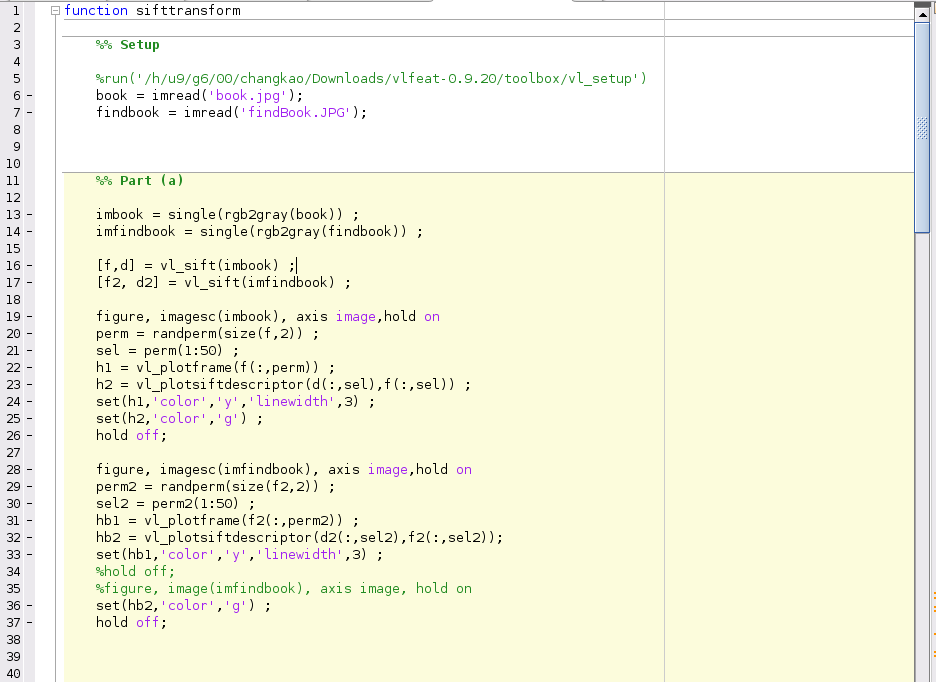
\includegraphics[width=1.35\textwidth]{img/2a1-code.png}
\caption{setup and 2a matlab code}
\end{figure}
\begin{figure}[h!]
\centering
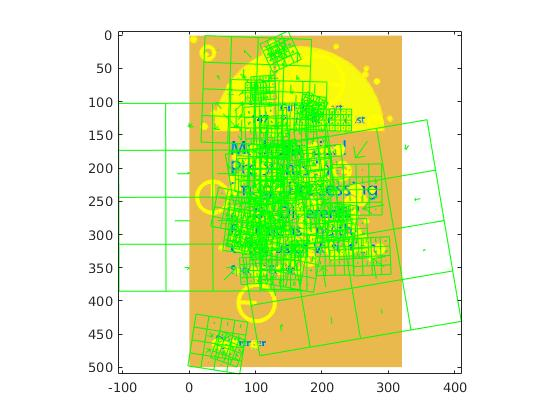
\includegraphics[width=1.35\textwidth]{img/2a1.jpg}
\caption{feature and keypoints on book.jpg}
\end{figure}
\begin{figure}[h!]
\centering
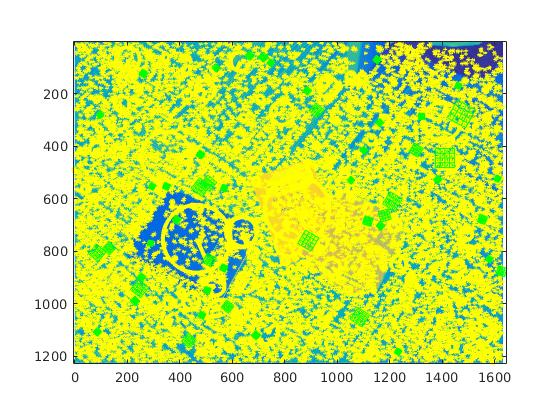
\includegraphics[width=1.35\textwidth]{img/2a2.jpg}
\caption{feature and keypoints on findBook.JPG}
\end{figure}


\begin{figure}[h!]
\centering
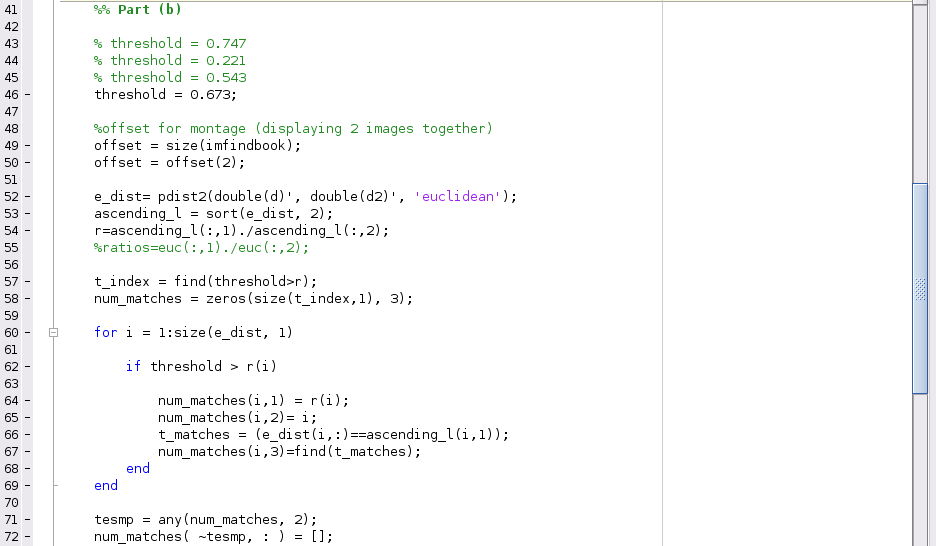
\includegraphics[width=1.35\textwidth]{img/2b1-code.png}
\caption{2b part 1 Matlab code}
\end{figure}
\begin{figure}[h!]
\centering
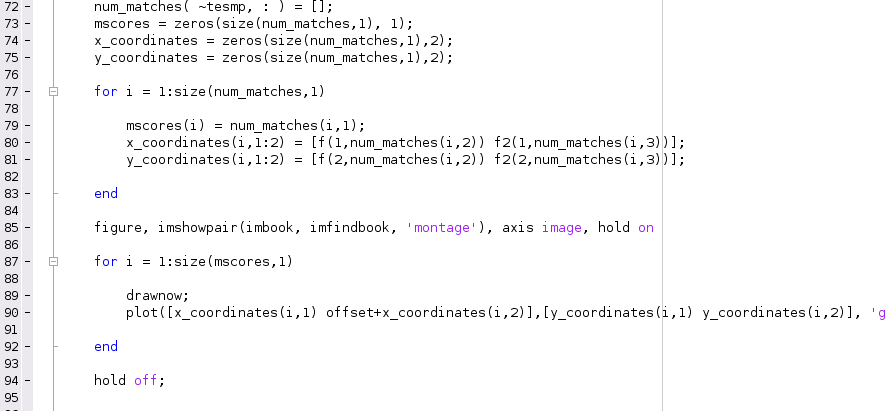
\includegraphics[width=1.35\textwidth]{img/2b2-code.png}
\caption{2b part 2}
\end{figure}
\begin{figure}[h!]
\centering
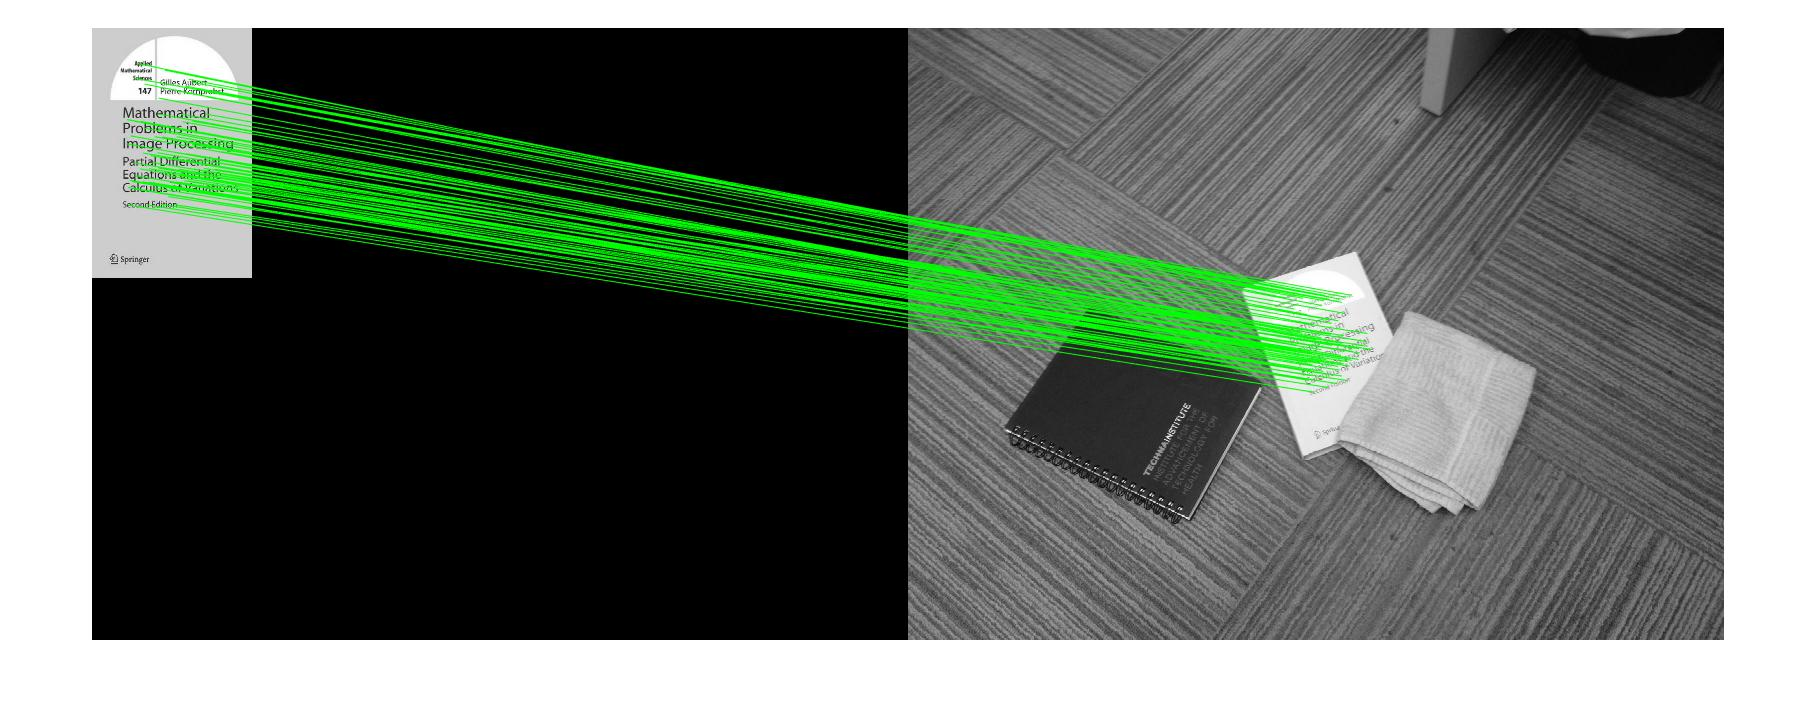
\includegraphics[width=1.35\textwidth]{img/2b.jpg}
\caption{output, threshold = 0.673}
\end{figure}
\begin{figure}[h!]
\centering
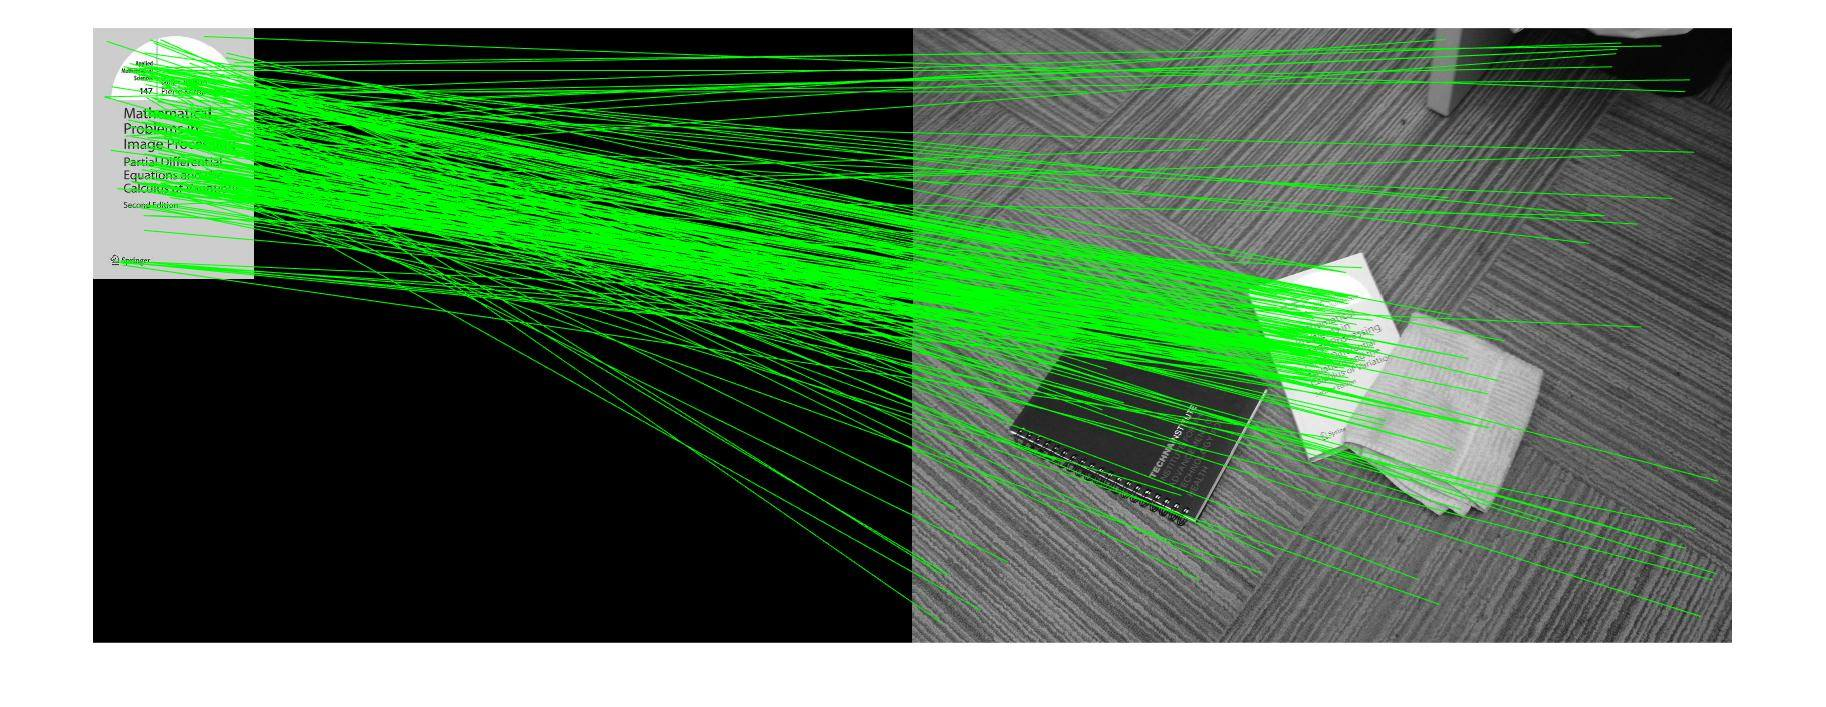
\includegraphics[width=1.35\textwidth]{img/2b-t098.jpg}
\caption{output, threshold = 0.98}
\end{figure}
\begin{figure}[h!]
\centering
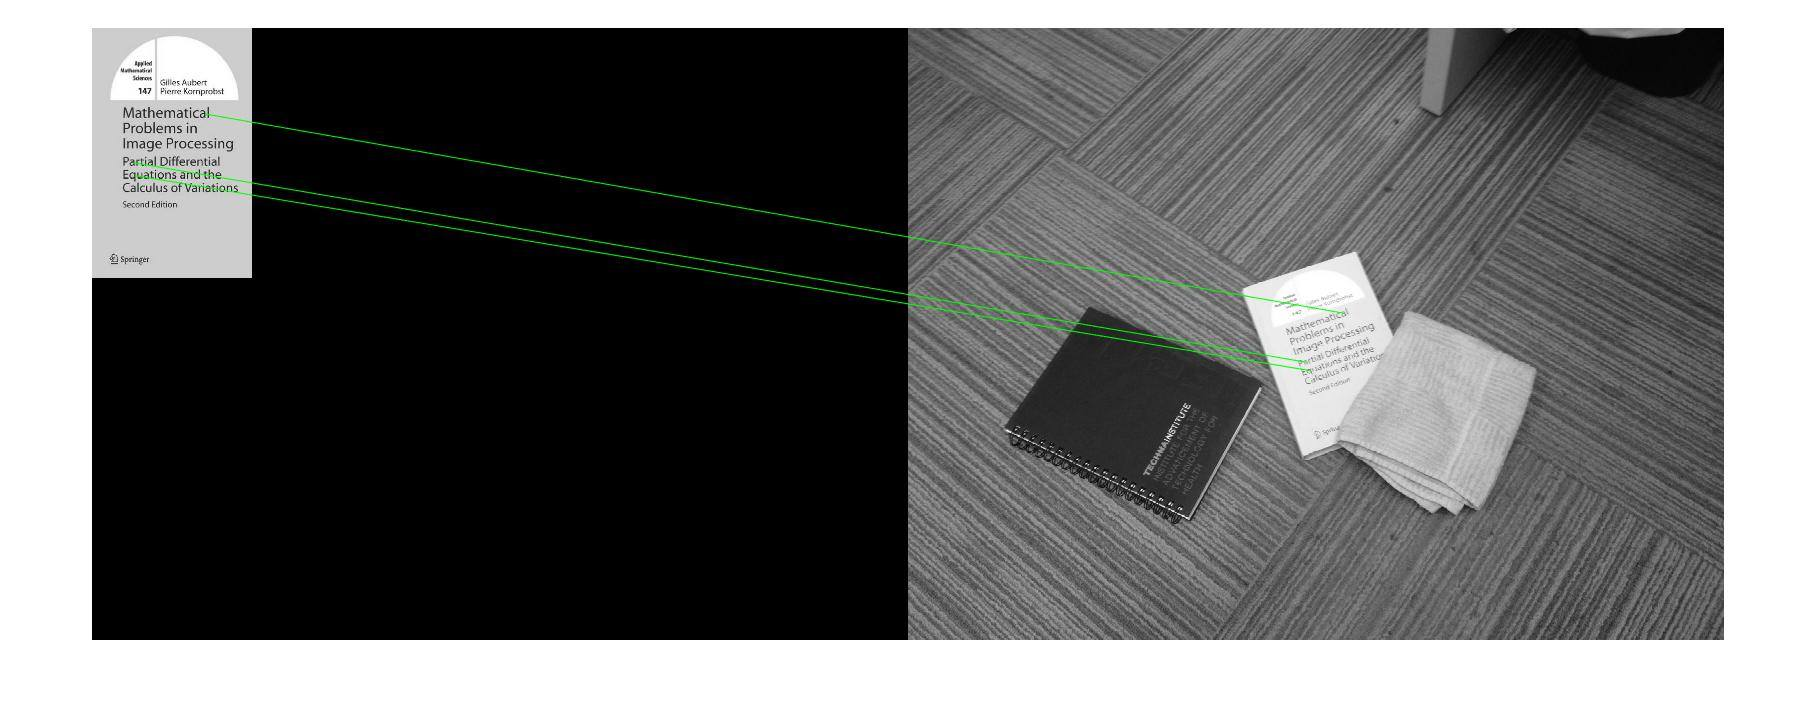
\includegraphics[width=1.35\textwidth]{img/2b-t0275.jpg}
\caption{output, threshold = 0.275}
\end{figure}


\begin{figure}[h!]
\centering
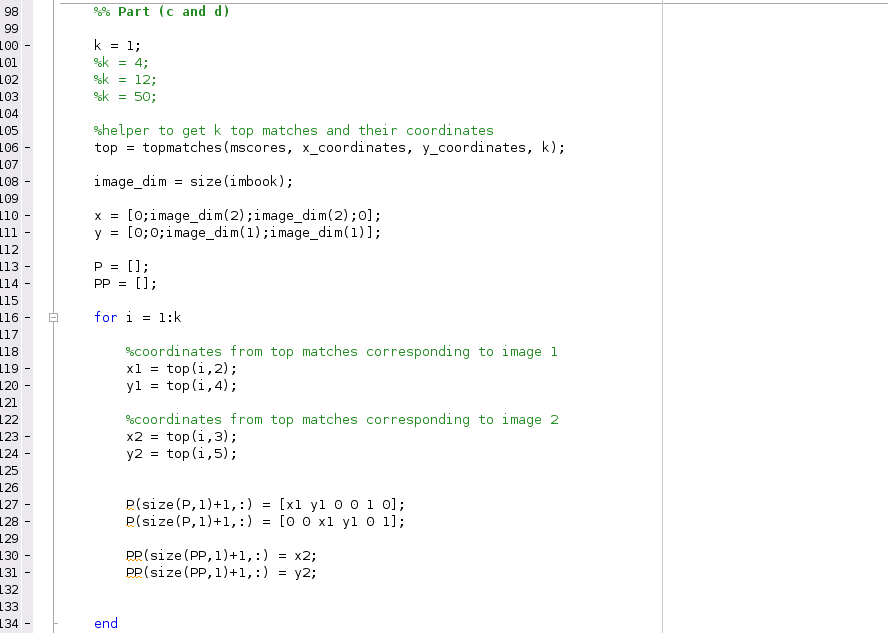
\includegraphics[width=1.35\textwidth]{img/2c1-code.png}
\caption{2c/d part 1 Matlab Code}
\end{figure}
\begin{figure}[h!]
\centering
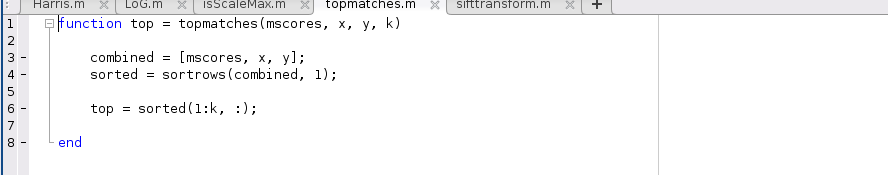
\includegraphics[width=1.35\textwidth]{img/2c2-code.png}
\caption{2c/d helper - topmatches }
\end{figure}
\begin{figure}[h!]
\centering
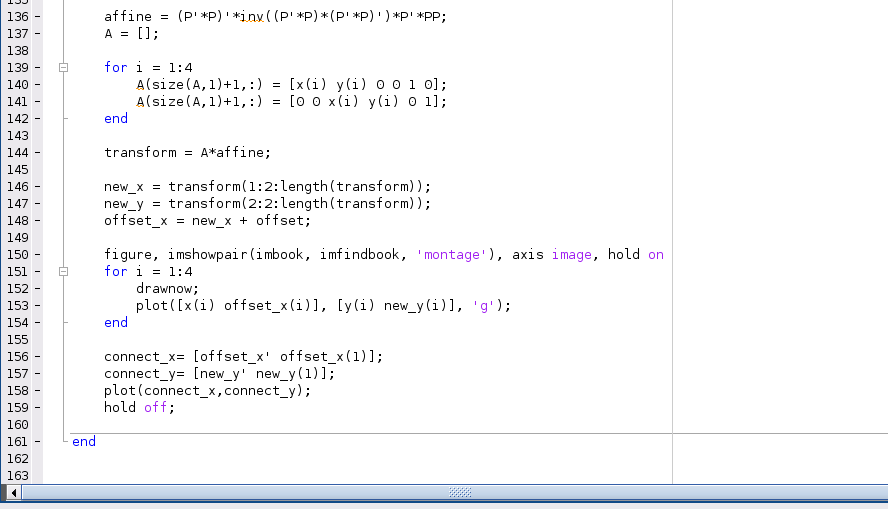
\includegraphics[width=1.35\textwidth]{img/2c3-code.png}
\caption{2c/d part 2}
\end{figure}



\begin{figure}[h!]
\centering
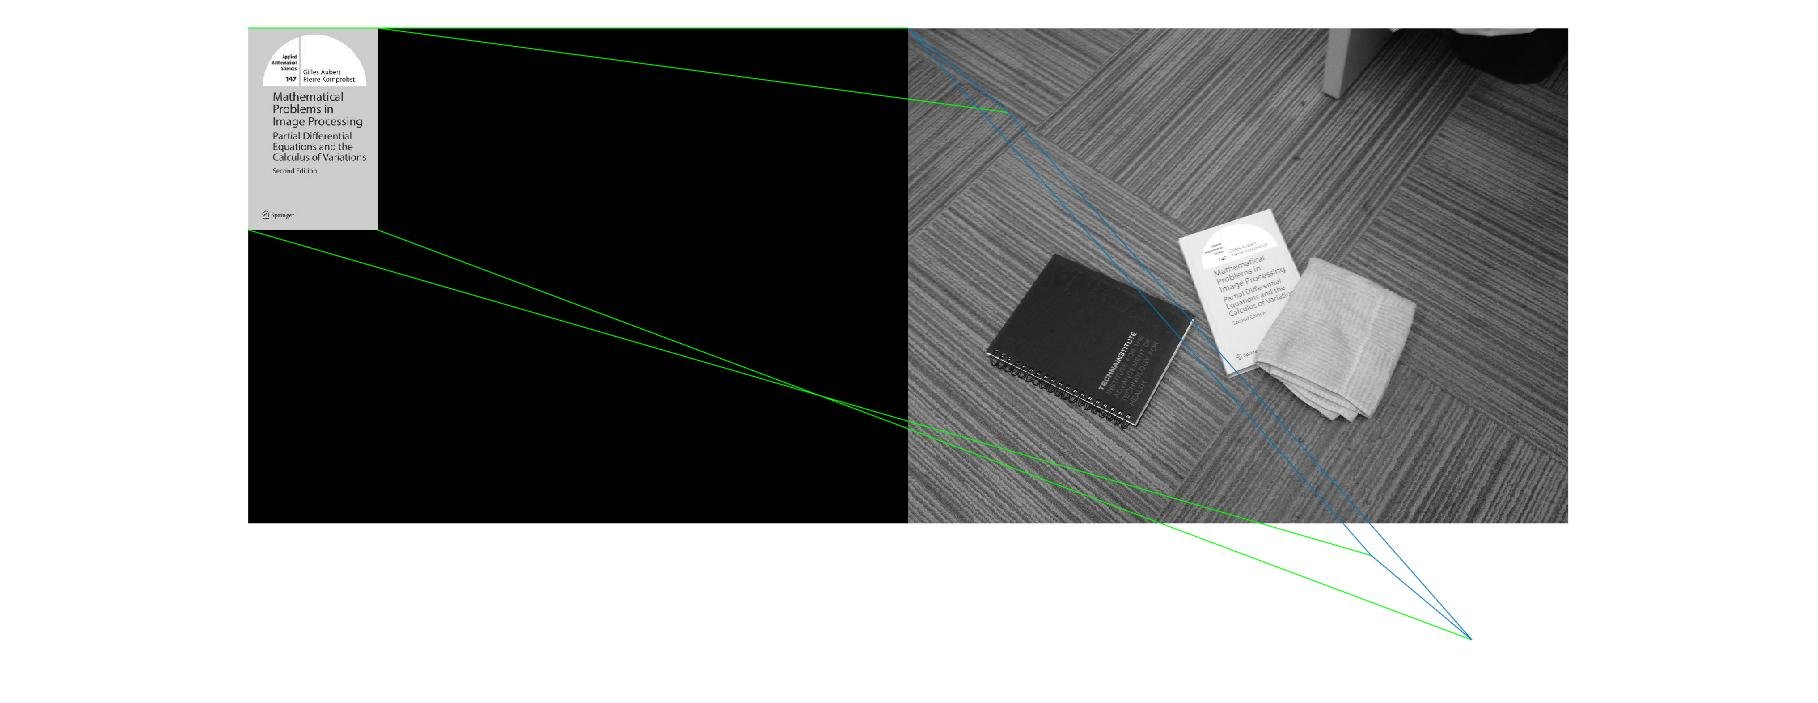
\includegraphics[width=1.35\textwidth]{img/2c-k1.jpg}
\caption{Affine transform w/ k=1}
\end{figure}
\begin{figure}[h!]
\centering
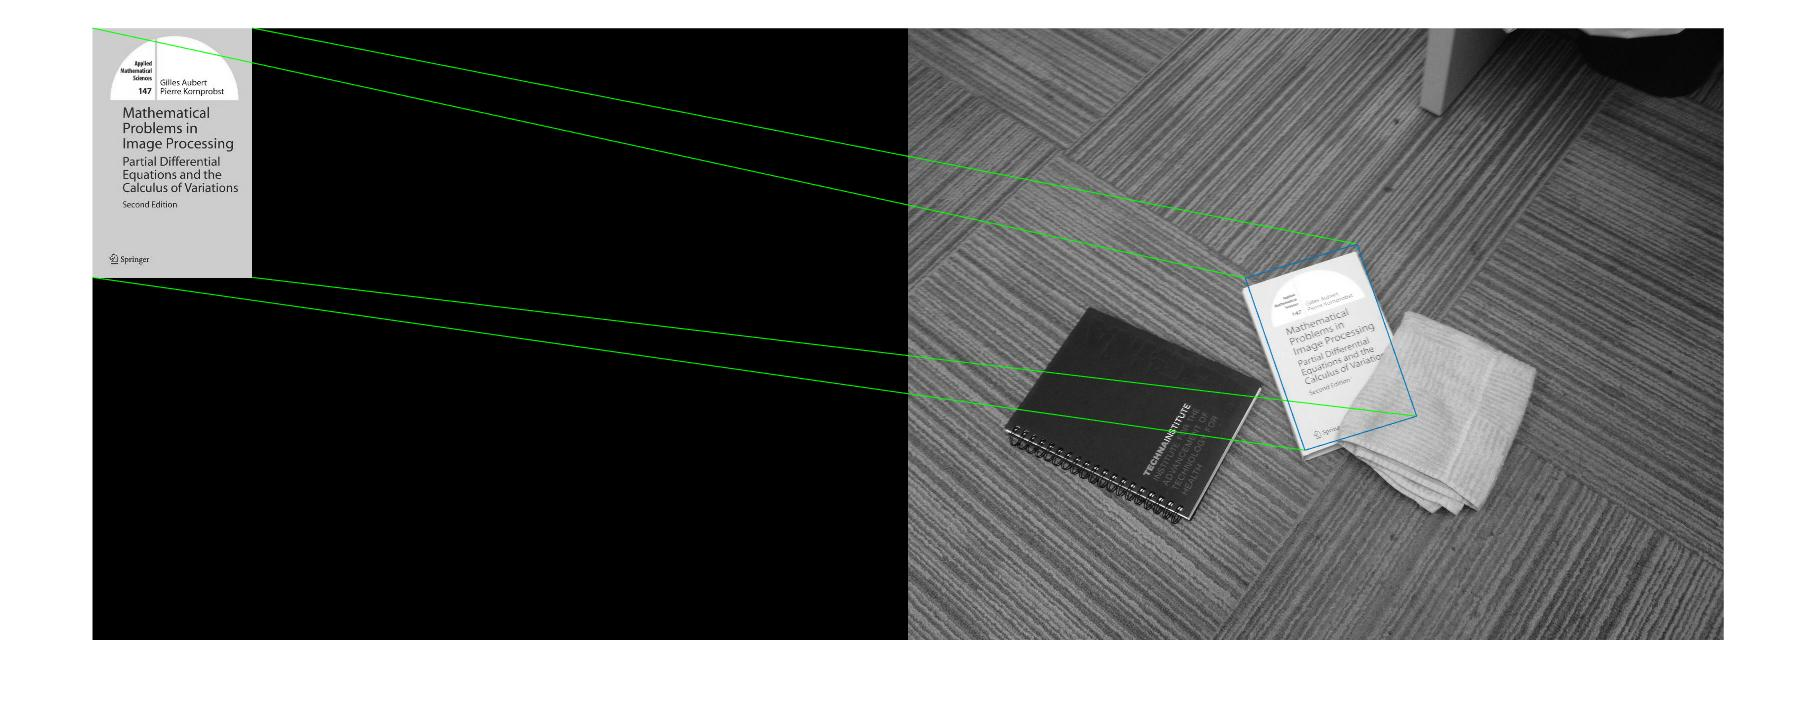
\includegraphics[width=1.35\textwidth]{img/2c-k4.jpg}
\caption{Affine transform w/ k=4}
\end{figure}
\begin{figure}[h!]
\centering
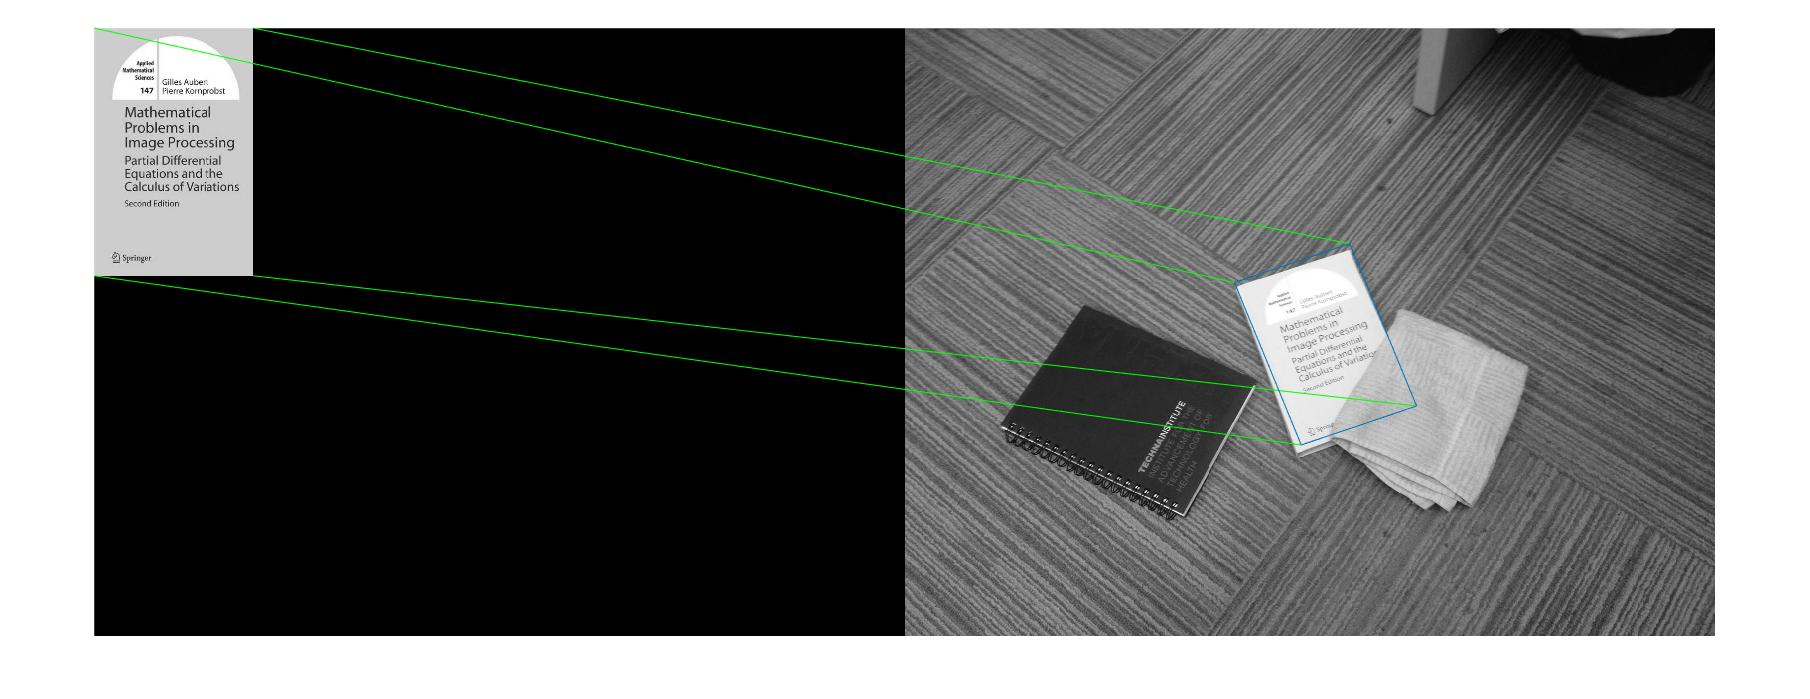
\includegraphics[width=1.35\textwidth]{img/2c-k12.jpg}
\caption{Affine transform w/ k=12}
\end{figure}
\begin{figure}[h!]
\centering
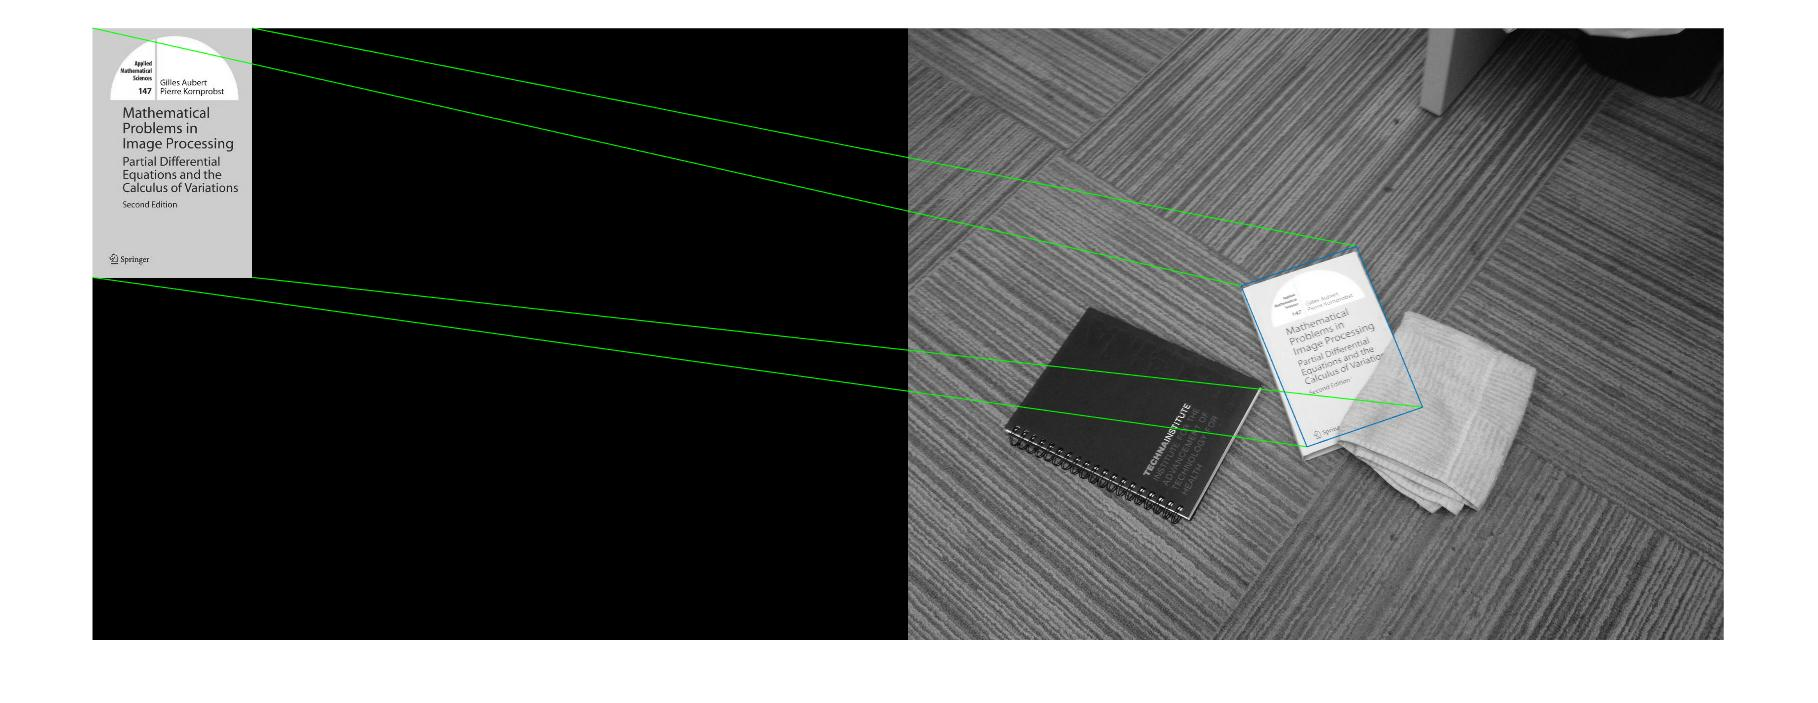
\includegraphics[width=1.35\textwidth]{img/2c-k50.jpg}
\caption{Affine transform w/ k=50}
\end{figure}


\end{document}
